\newpage
\begin{flushleft}
{\fontsize{16pt}{16pt}\selectfont \textbf{CHAPTER 6}}
\end{flushleft}		
\begin{center}
{\fontsize{18pt}{22pt}\selectfont \textbf{SYSTEM IMPLEMENTATION}}\\[2mm]
\end{center}
\addcontentsline{toc}{section}{\numberline{6}SYSTEM IMPLEMENTATION}

\onehalfspacing
\justifying
\noindent \textbf{6.1 INTRODUCTION} \\[2mm]
The implementation phase represents the practical realization of system architectural designs into a functional, production-ready enterprise software platform. For SmartCampus AI, this demanding engineering phase comprises multiple synchronized tasks: setting up edge camera streaming pipelines, embedding deep neural networks, configuring in-memory vector databases, authoring relational database schemas, and building responsive client portals. A core engineering challenge is ensuring seamless, low-latency inter-service communication across Python FastAPI, NestJS 11, PostgreSQL 16, Redis 7, and Next.js 16 so the platform can continuously execute real-time face detection, biometric verification, candidate clustering, conflict resolution, and behavioral alert streaming without frame drops or memory leaks.

\vspace{0.15in}
\noindent In the edge vision service (`apps/ai-service`), asynchronous frame decoders continuously ingest 1080p video from overhead IP cameras. SCRFD-10G isolates facial bounding boxes, while Laplacian variance kernels evaluate frame sharpness to discard motion-blurred artifacts. Aligned $112 \times 112$ crops are forwarded through ArcFace, extracting 512-dimensional continuous feature embeddings that are matched against an in-memory FAISS `IndexFlatIP` repository in sub-millisecond time. In parallel, the NestJS 11 API Gateway (`apps/api`) coordinates multi-tier authentication, manages session lifecycles, persists verified attendance ledgers to PostgreSQL 16 via Prisma ORM, and broadcasts live WebSocket telemetry. The modern Next.js 16 web portal (`apps/web`) renders glassmorphism dashboards with zero-refresh optimistic state updates.

\vspace{0.2in}
\noindent \textbf{6.2 IMPLEMENTATION OF CORE MODULES \& SYSTEM INTERFACES}

\begin{figure}[h]
    \centering
    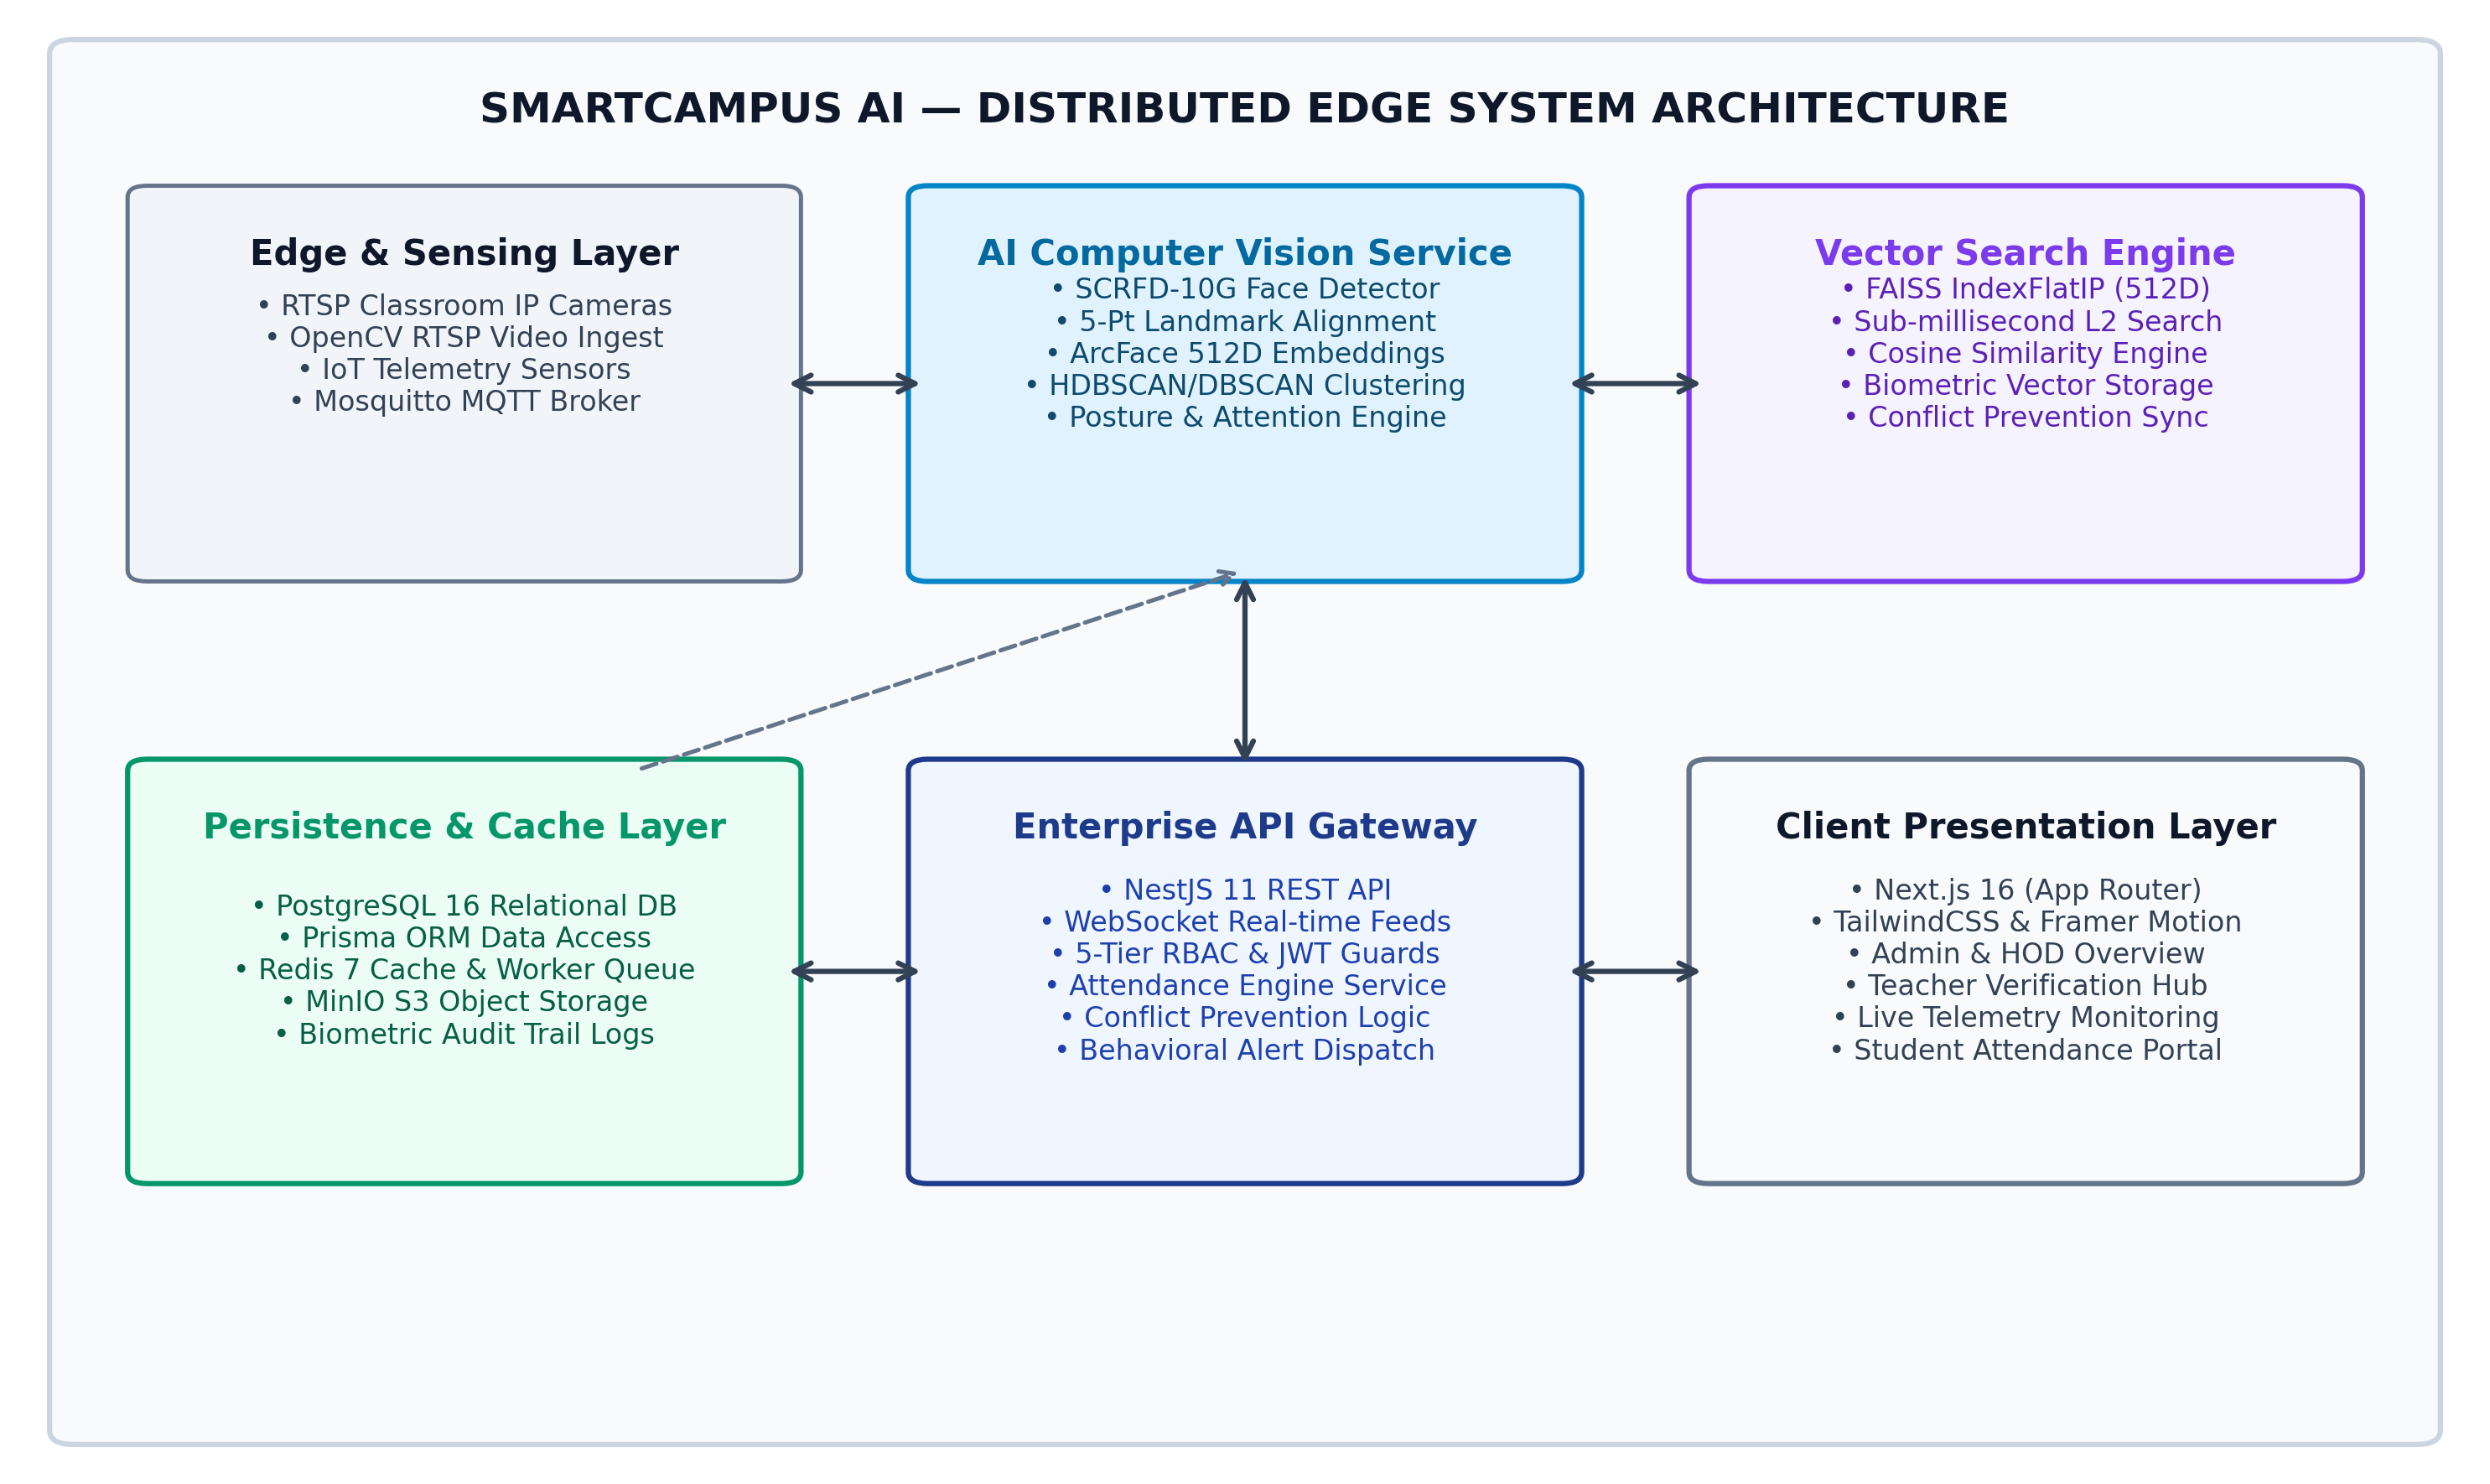
\includegraphics[width=0.88\textwidth]{assets/fig_architecture.png}
    \caption{Classroom 408 Prototype Deployment \& Optical Video Setup}
    \label{fig:impl_setup}
\end{figure}

\noindent Figure 6.1 illustrates the physical prototype deployment within Classroom 408 at Vemana Institute of Technology. The overhead Full HD IP dome camera overlooks the tiered student seating area, streaming real-time H.264 video at 25 FPS over RTSP to the localized edge inference server.

\begin{figure}[h]
    \centering
    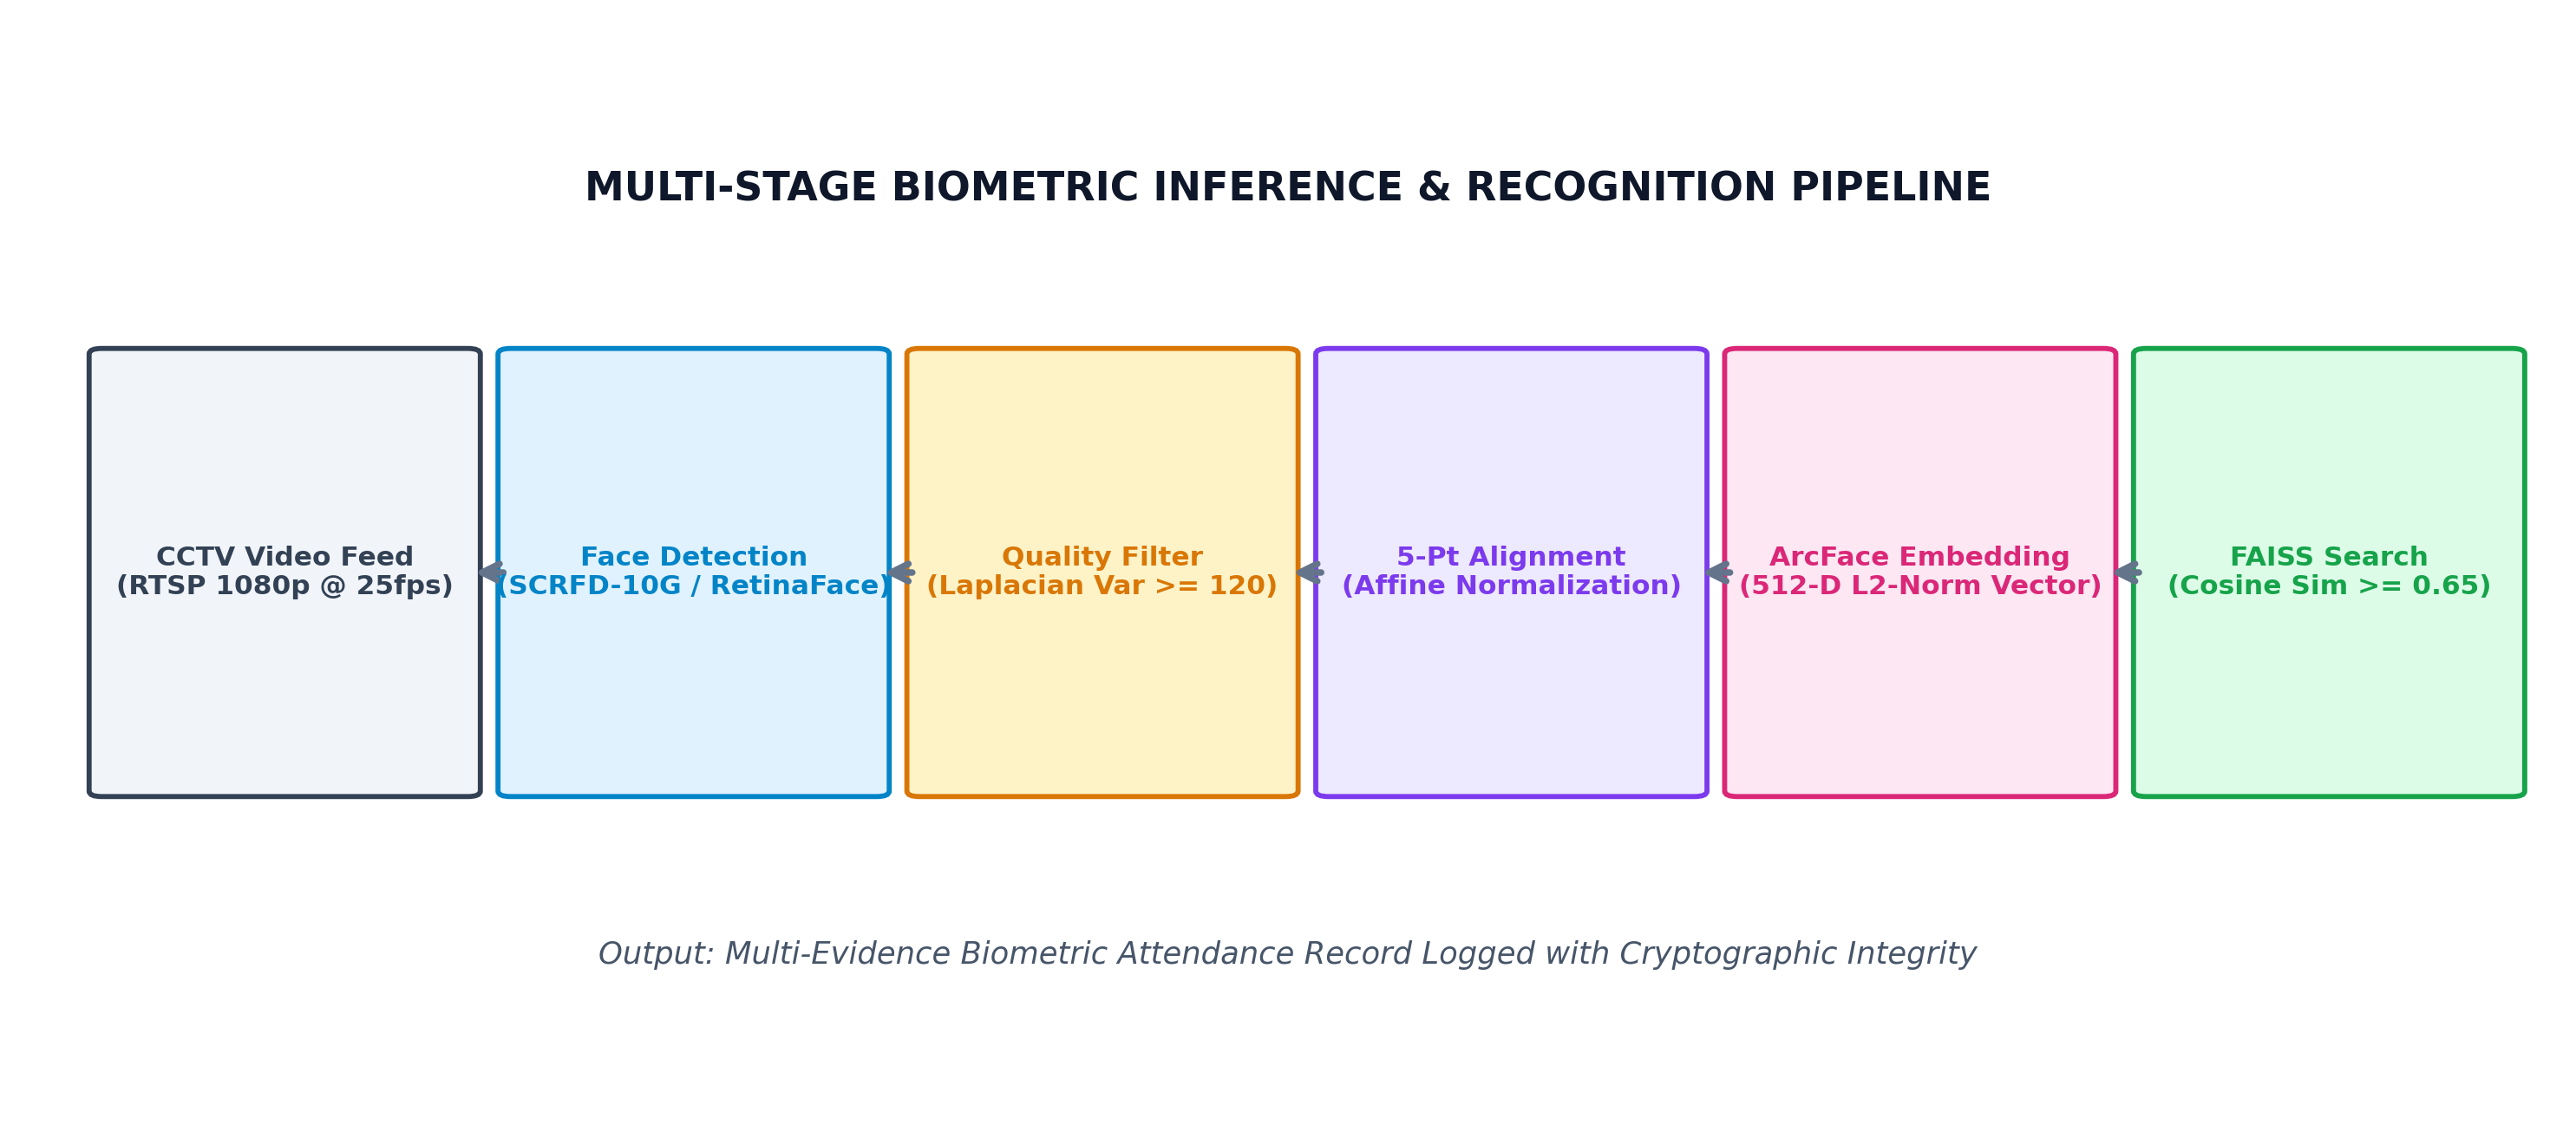
\includegraphics[width=0.92\textwidth]{assets/fig_pipeline.png}
    \caption{Multi-Stage Biometric Face Recognition Pipeline Implementation}
    \label{fig:impl_pipeline}
\end{figure}

\noindent Figure 6.2 illustrates the multi-stage neural vision pipeline operating in memory: raw video frames are decoded, filtered via Laplacian variance ($\sigma^2_\Delta \ge 120.0$), aligned using 5-point affine transforms, embedded into 512D unit vectors via ArcFace, and matched against FAISS index vectors in under 1.5 milliseconds.

\begin{figure}[h]
    \centering
    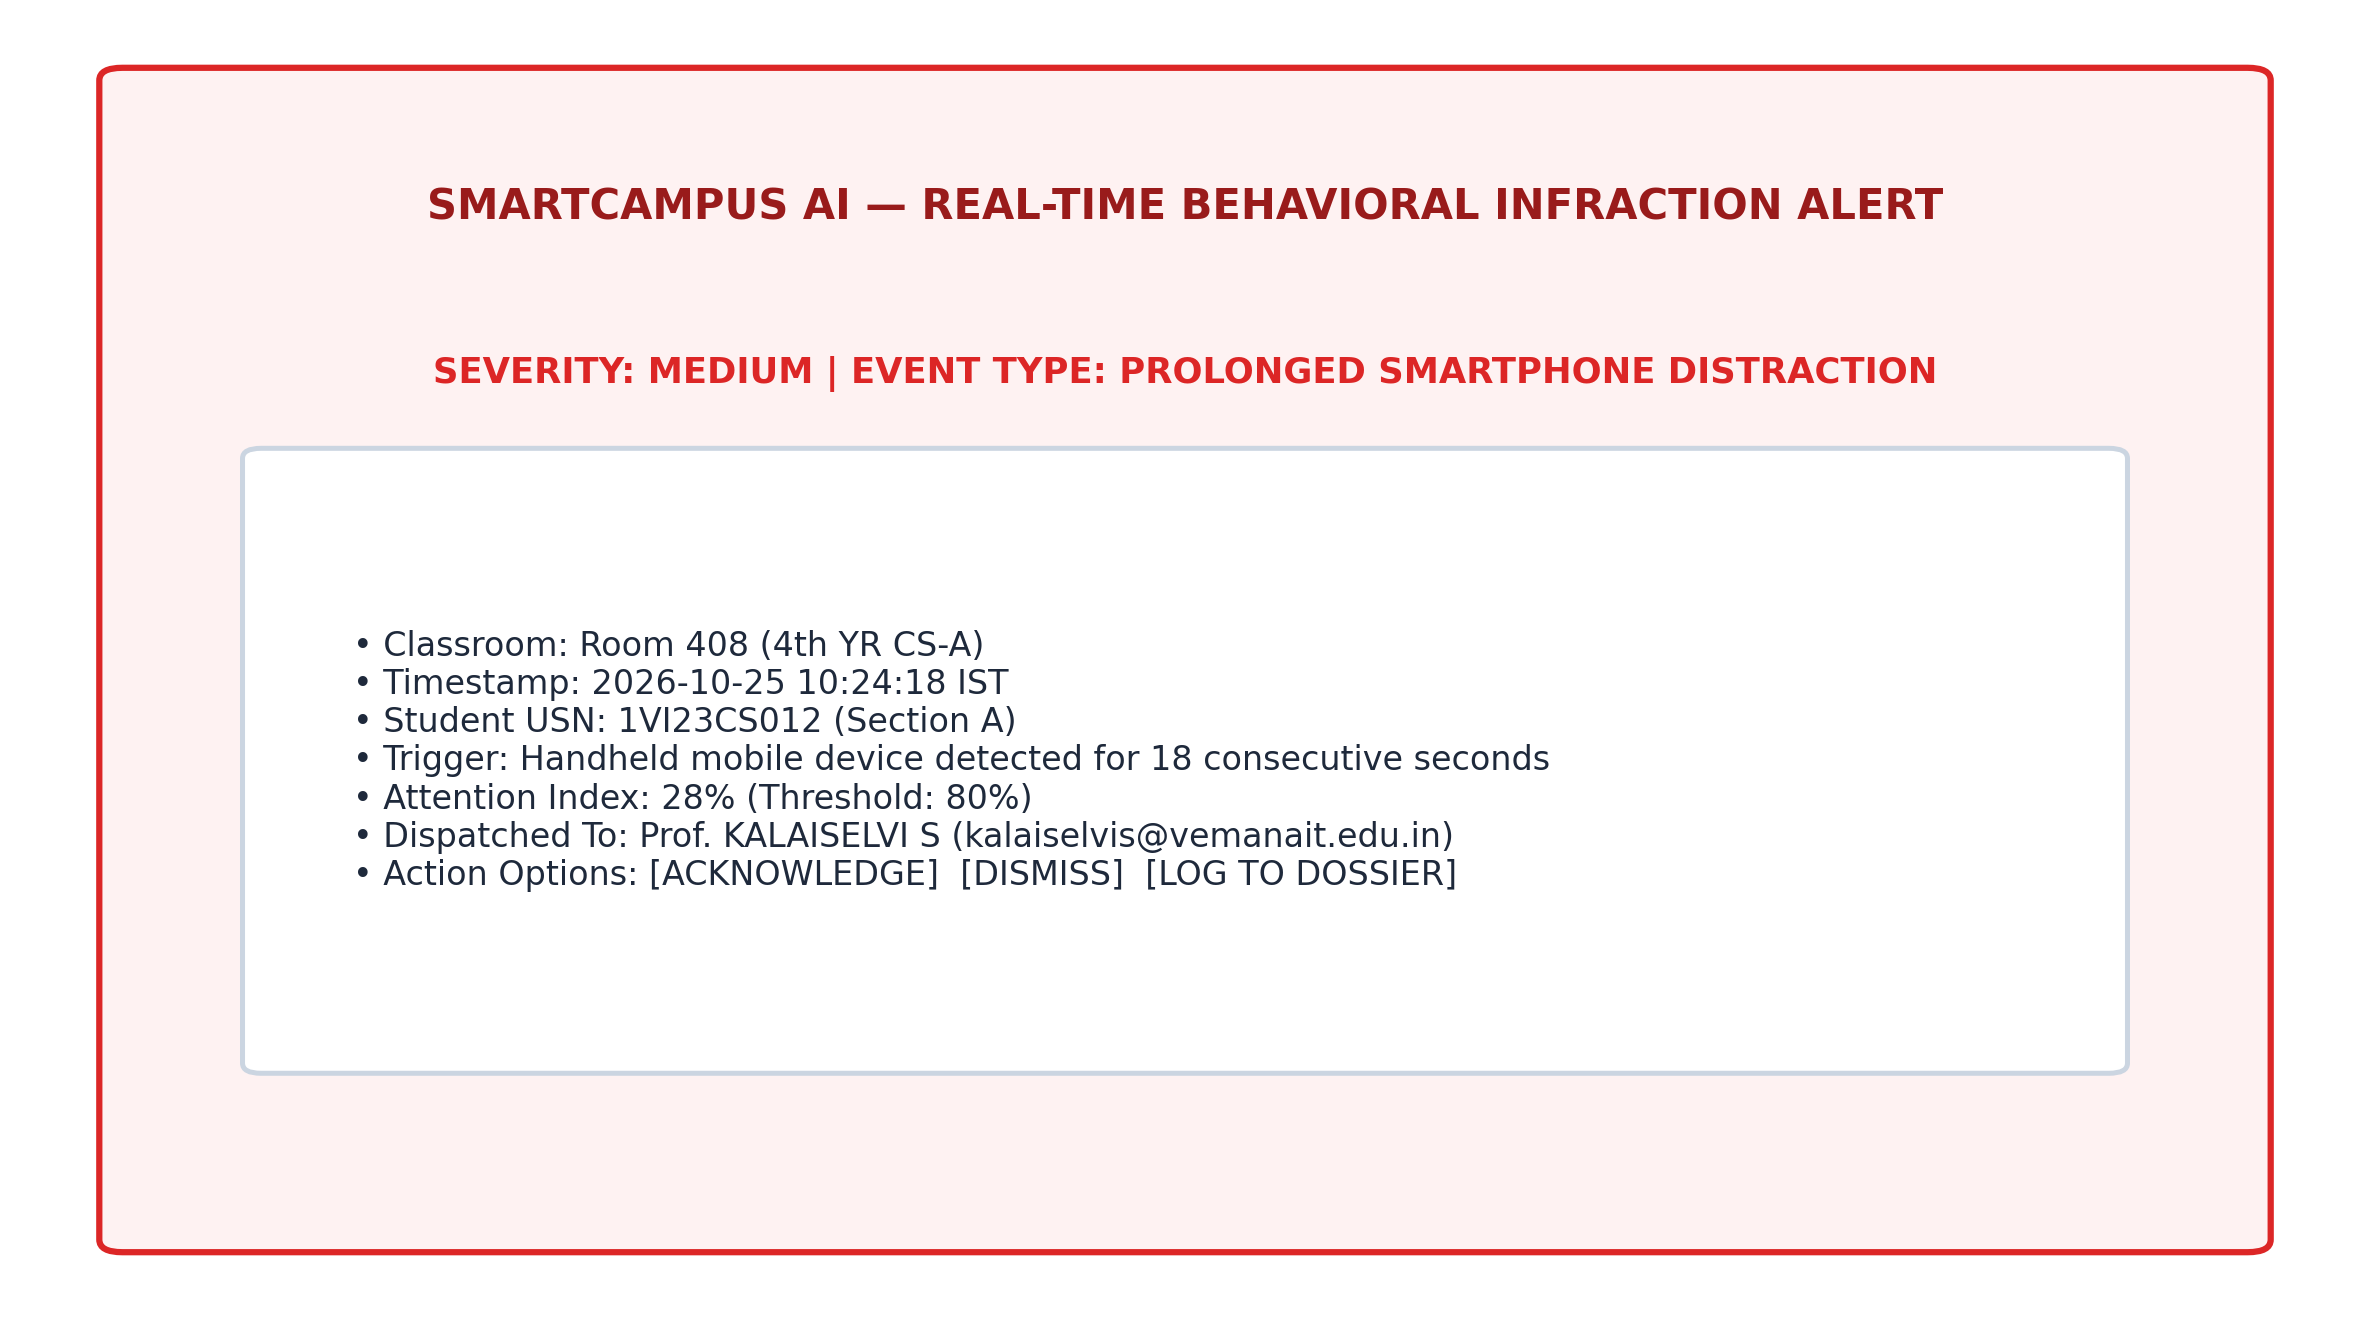
\includegraphics[width=0.85\textwidth]{assets/fig_behavior_alert.png}
    \caption{Automated In-Class Behavioral Alert \& Push Telemetry Notice}
    \label{fig:impl_alert}
\end{figure}

\noindent Figure 6.3 illustrates an automated in-class behavioral alert generated by the SmartCampus AI vision engine and pushed via WebSockets to the course instructor's dashboard. The alert specifies student identity (`1VI23CS012`), classroom location (`Room 408`), infraction type (prolonged mobile phone distraction), and Attention Index score ($28\%$), allowing faculty to intervene or log the event to student dossiers.

\begin{figure}[h]
    \centering
    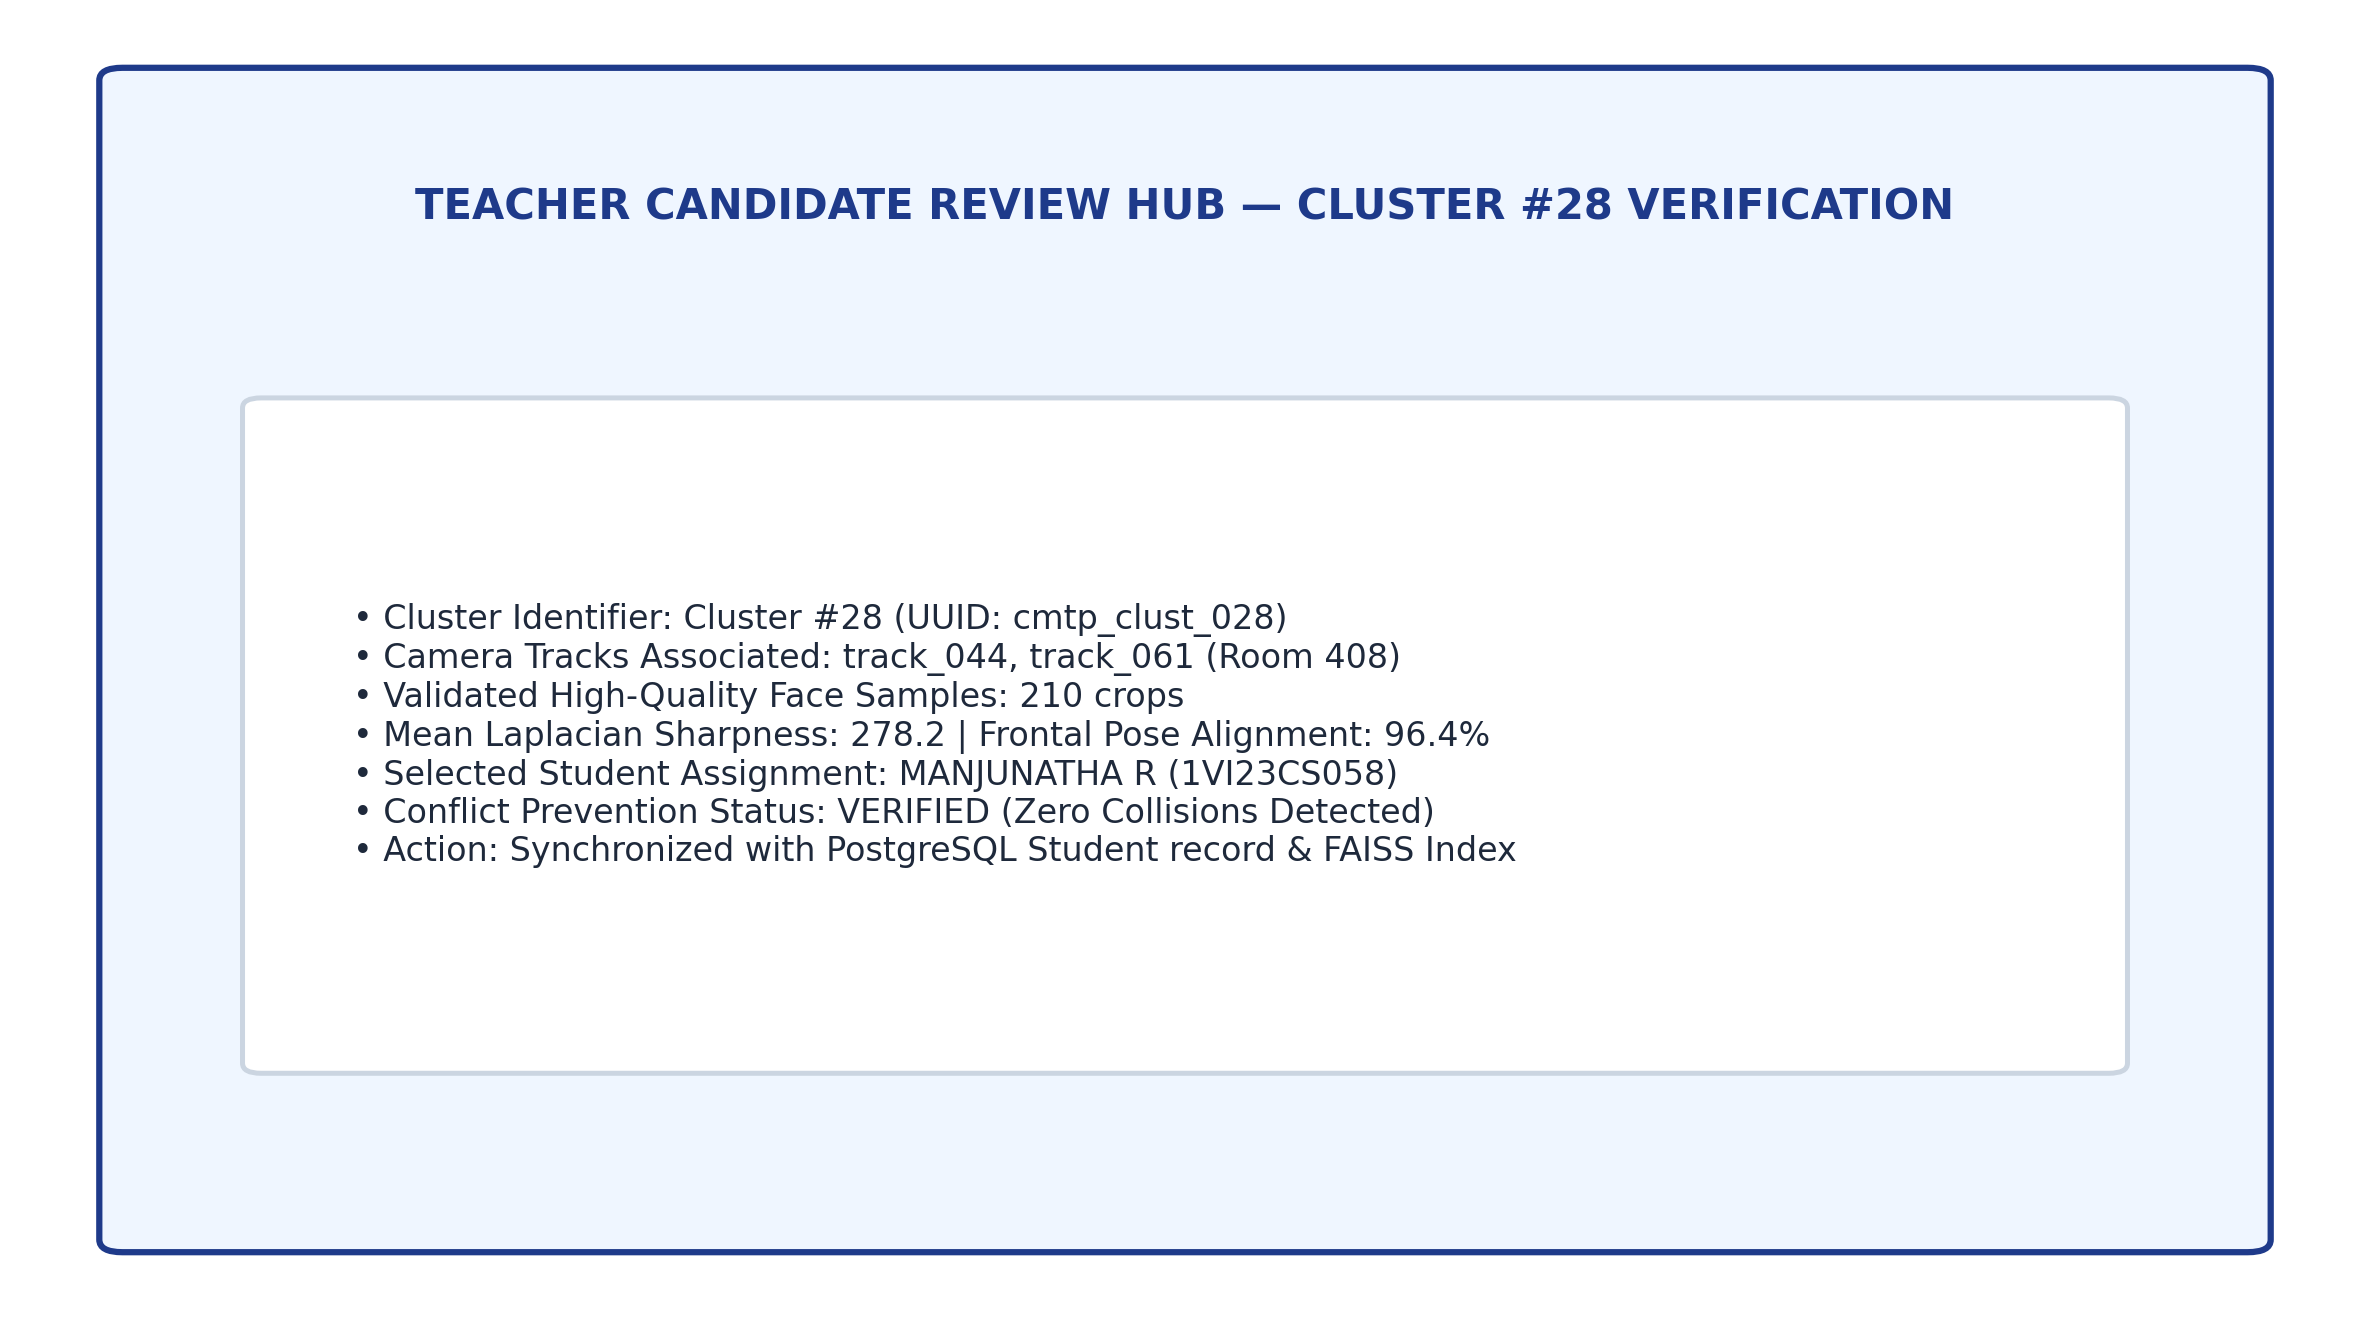
\includegraphics[width=0.85\textwidth]{assets/fig_candidate_review.png}
    \caption{Teacher Candidate Review Hub \& Conflict Resolution Interface}
    \label{fig:impl_review}
\end{figure}

\noindent Figure 6.4 depicts the Teacher Candidate Review Hub card for Cluster \#28. The interface displays validated sample counts (210 crops), representative crop sharpness, candidate student selection, and conflict prevention status. When verified, the assignment is synchronized atomically across PostgreSQL and FAISS.

\begin{figure}[h]
    \centering
    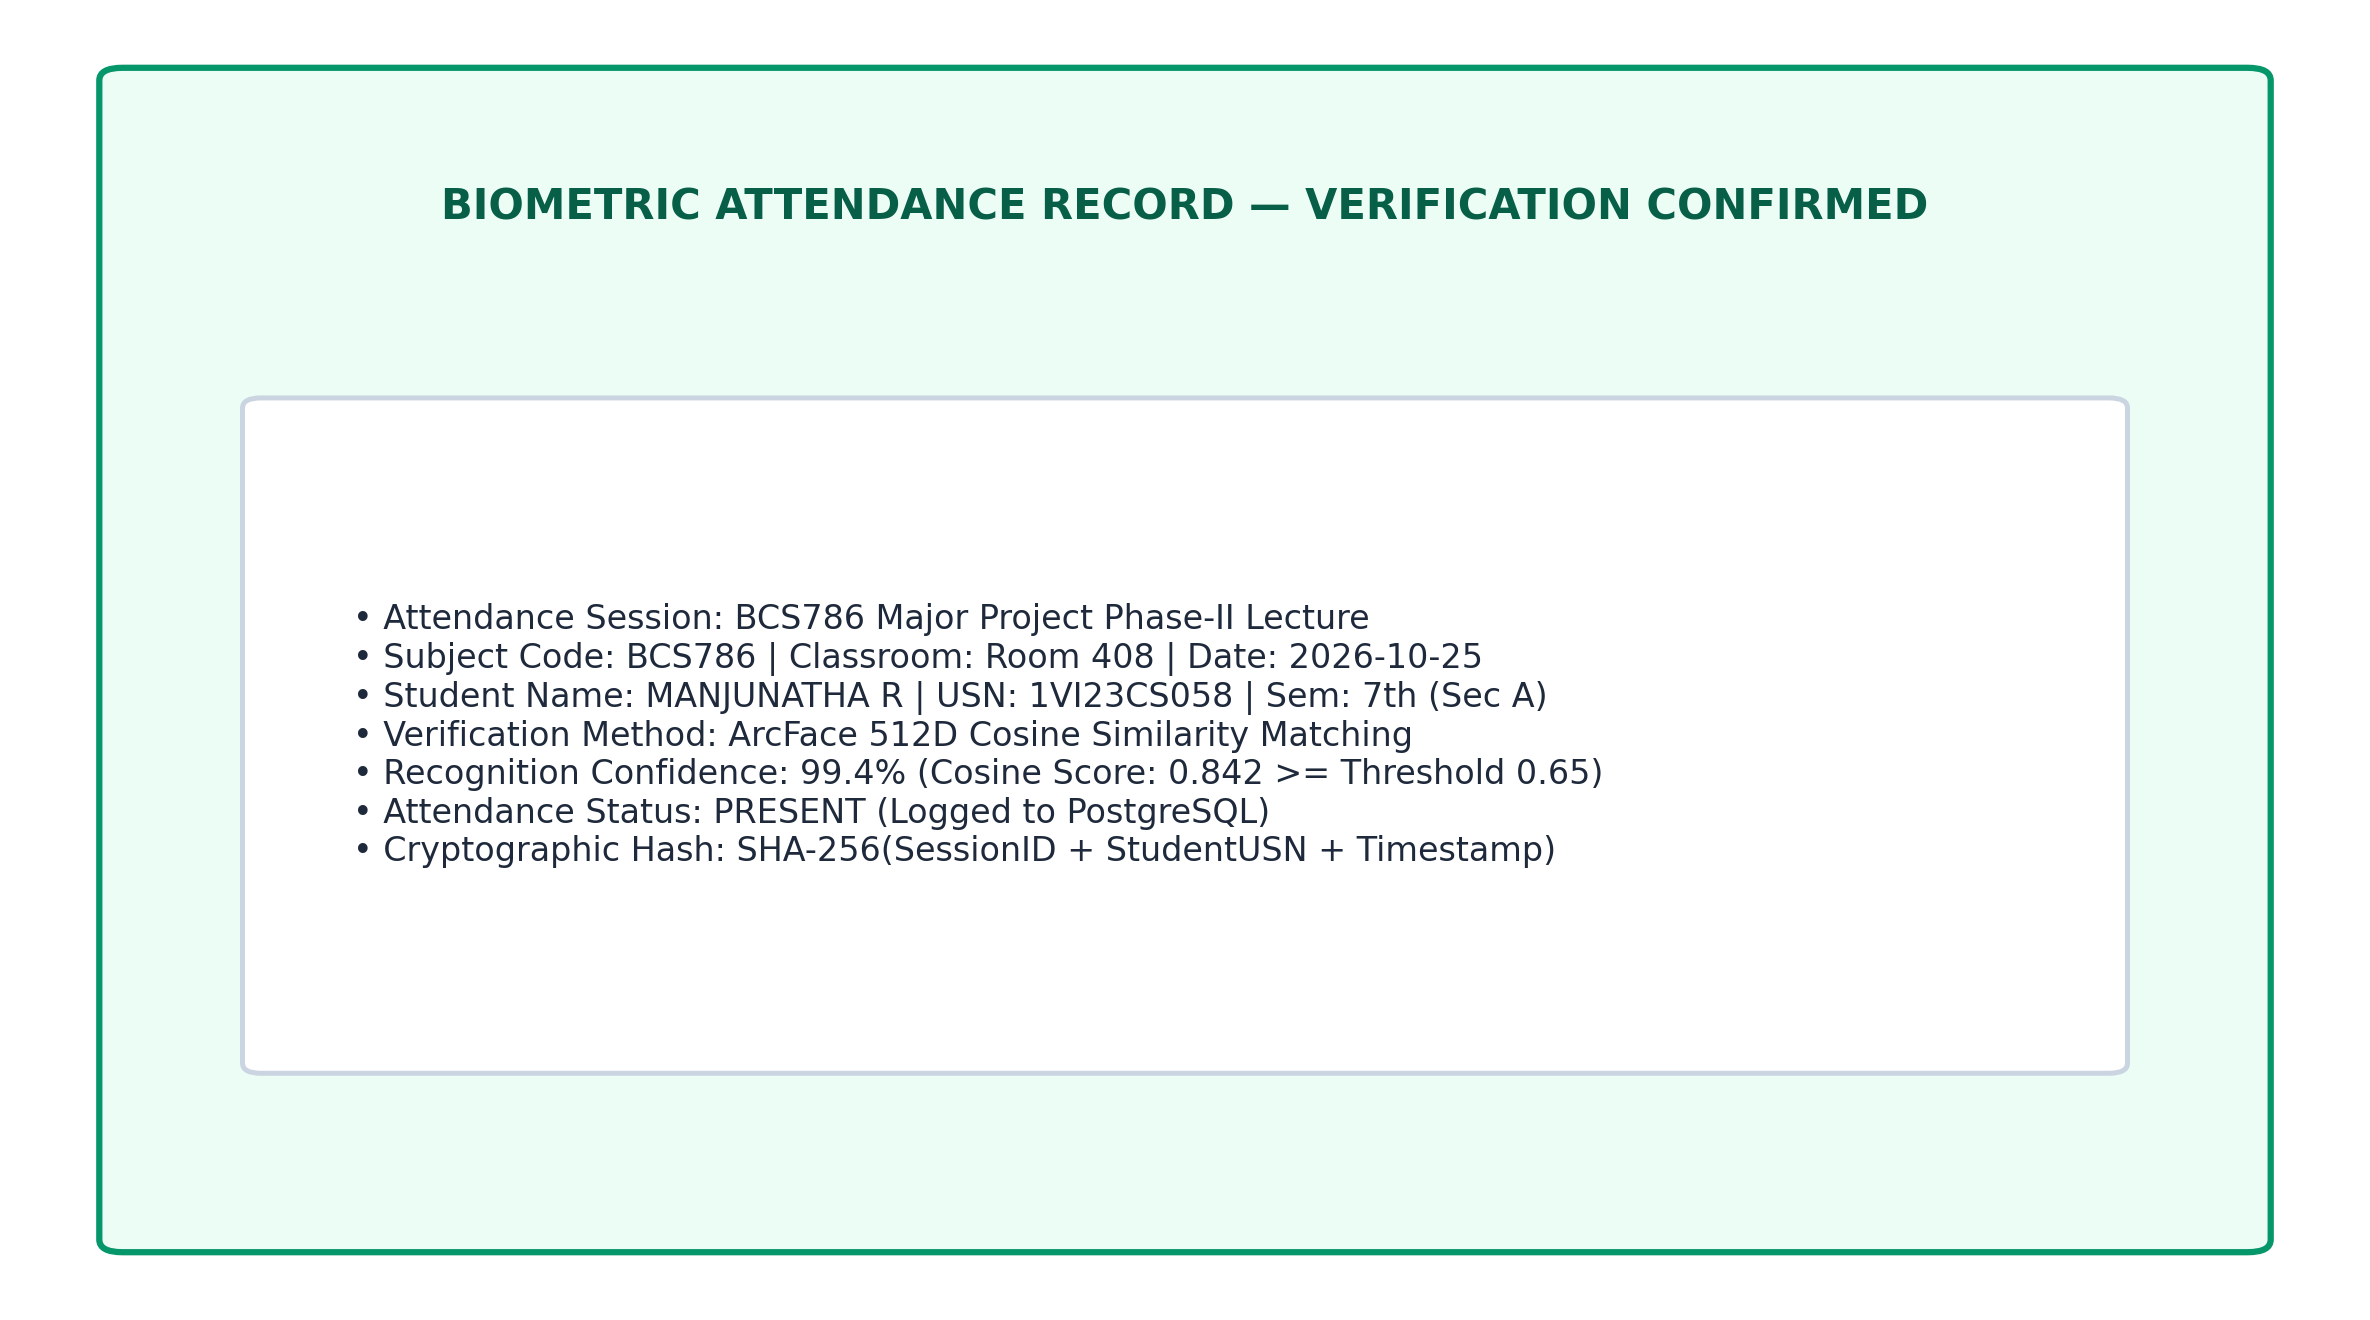
\includegraphics[width=0.85\textwidth]{assets/fig_attendance_receipt.png}
    \caption{Biometric Attendance Verification Confirmation Receipt}
    \label{fig:impl_receipt}
\end{figure}

\noindent Figure 6.5 illustrates the cryptographic biometric attendance verification receipt generated upon positive ArcFace similarity matching (cosine score $0.842 \ge 0.65$), confirming student attendance for the active lecture session.

\begin{figure}[h]
    \centering
    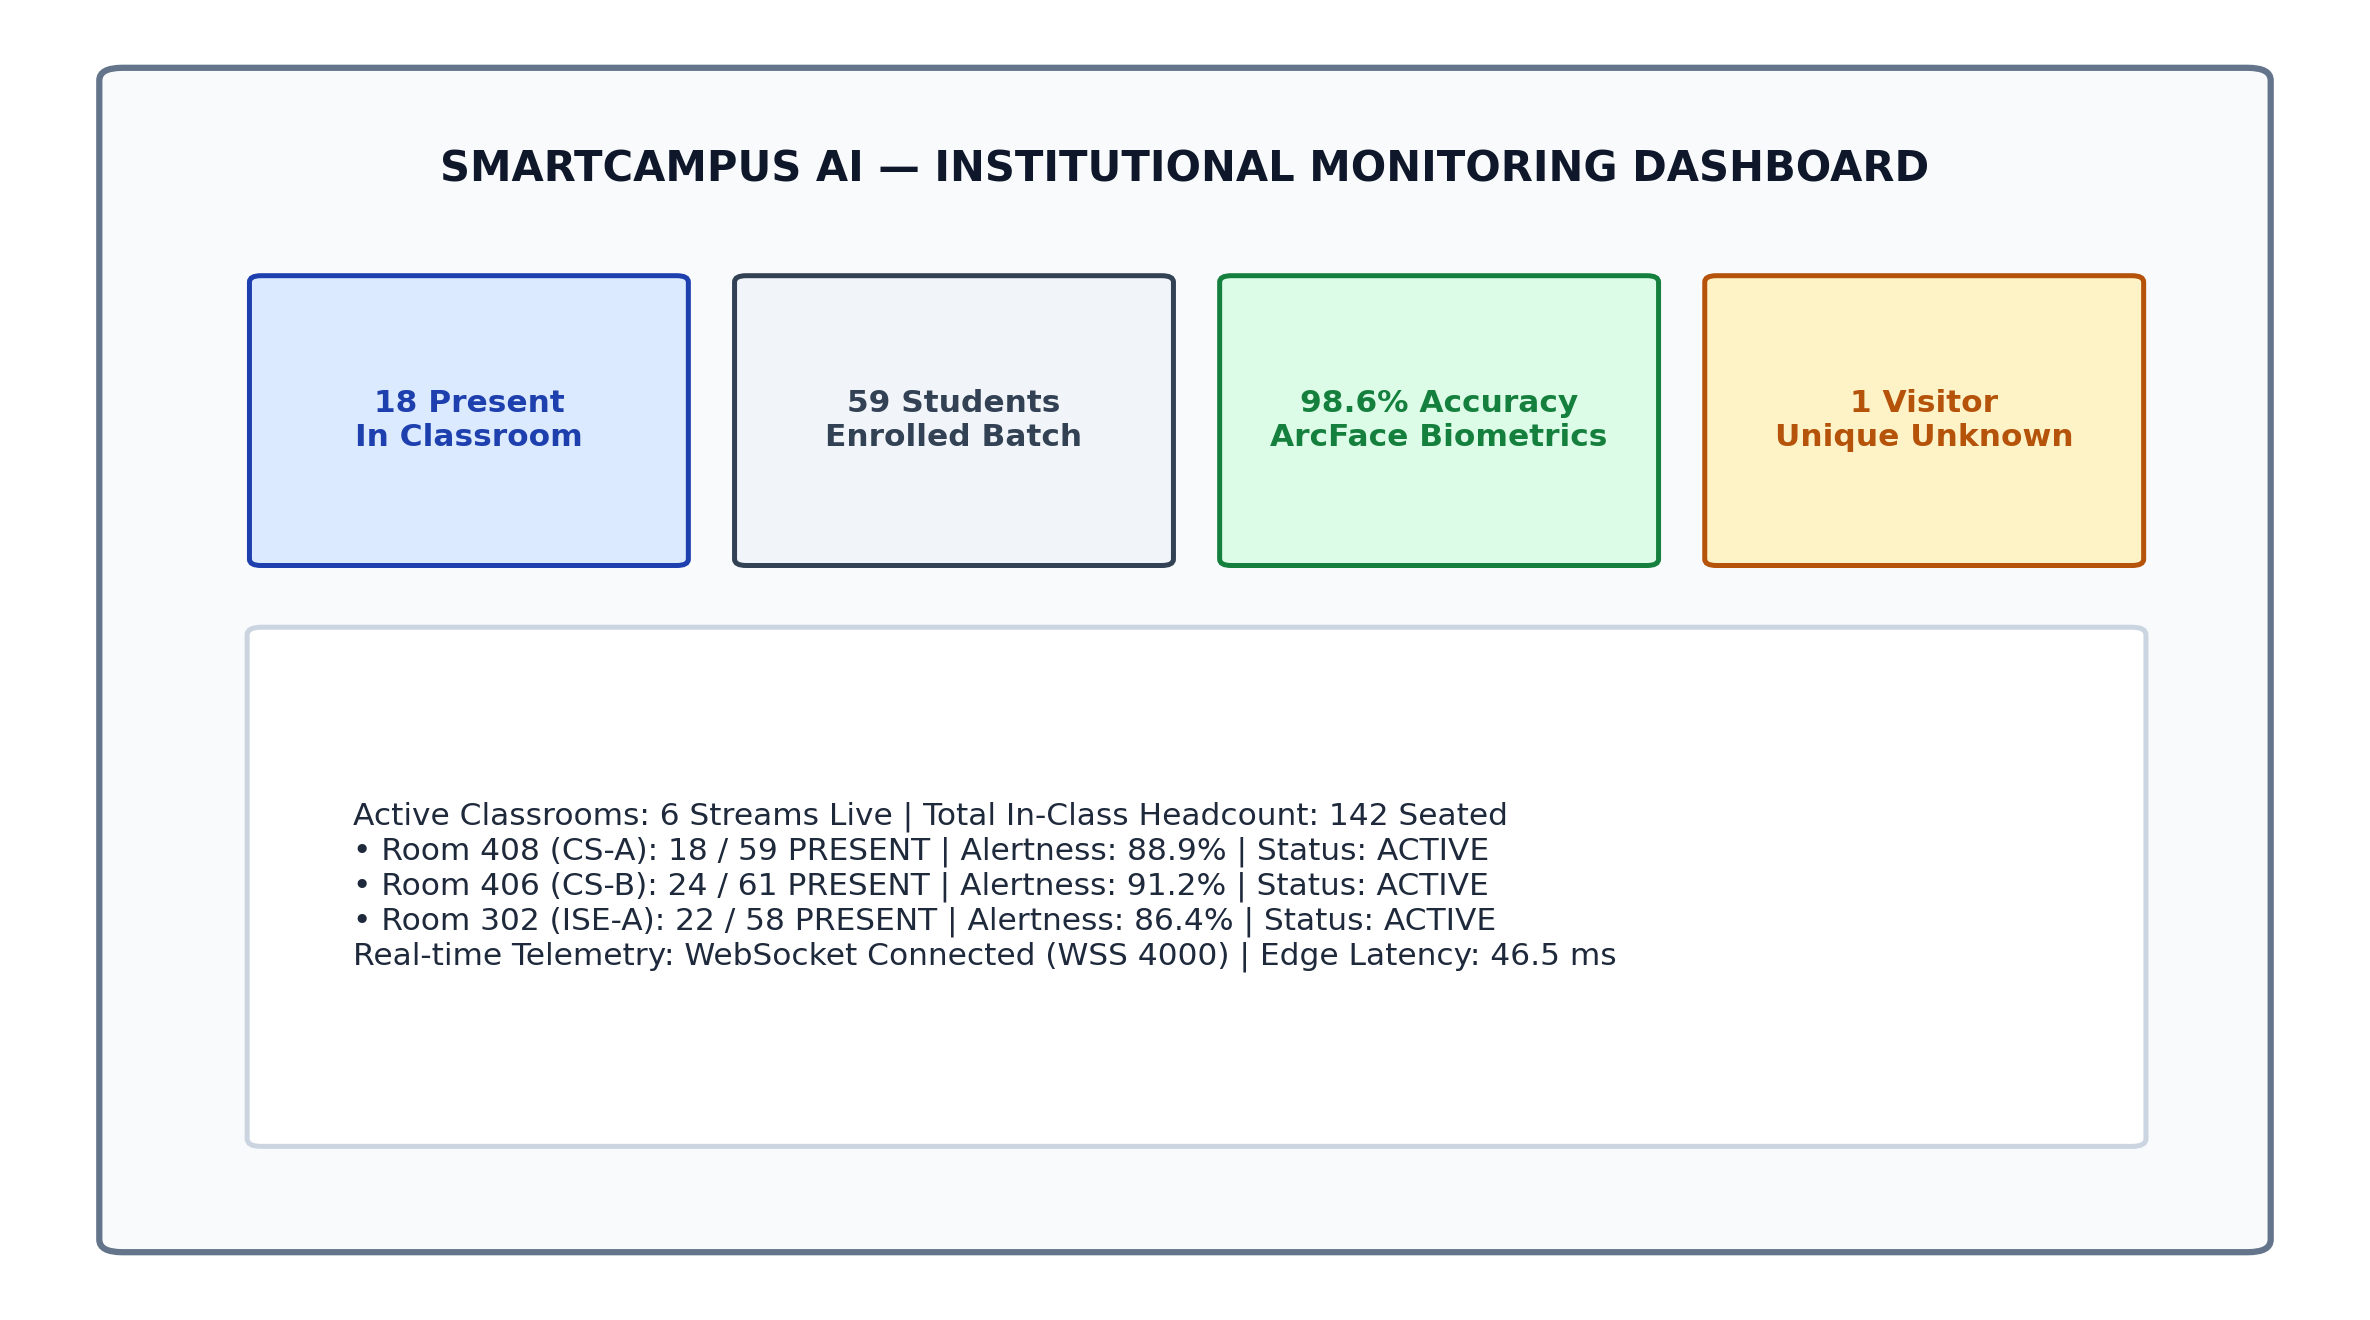
\includegraphics[width=0.85\textwidth]{assets/fig_admin_dashboard.png}
    \caption{SmartCampus AI Institutional Admin \& HOD Monitoring Dashboard}
    \label{fig:impl_dash}
\end{figure}

\noindent Figure 6.6 illustrates the SmartCampus AI Admin and HOD Dashboard, rendering normalized headcount metrics (18 Present in Room / 59 Enrolled Batch), active classroom video feeds, departmental alertness scores (88.9\%), and real-time edge processing latency (46.5 ms).
\newpage
